\section{Lehramt Primarstufe und Sekundarstufe I und Lehramt an der
Sonderschule}

Hier nun ein paar grundlegende Informationen für Studierende des Lehramts der
Primar- und Sekundarstufe I und des Lehramts der Sonderschule: Auch nach der
Umstellung auf Bachelor- und Master-Studiengänge gibt es für Euch einen eigenen
Studiengang, der weitestgehend losgelöst von den Bachelor- und anderen
Lehramts-Studierenden ist. Im ersten Studienabschnitt, dem Bachelor, müsst ihr
im Pflichtbereich insgesamt sieben Module absolvieren, also insgesamt 45 LP.
Diese Module sind: \emphm{Grundlagen der Mathematik} (M1), \emphm{Grundbildung
Lineare Algebra} (M2), \emphm{Grundbildung Analysis} (M3) (je 4 SWS Vorlesungen
und 2 SWS Übungen, 9 LP), \emphm{Grundbildung Geometrie} (GG),
\emphm{Grundbildung Stochastik} (GS) (je 2+1 SWS, 5 LP) und ein
\emphm{Softwarepraktikum} (EMS) (2 SWS, 4 LP). Außerdem müsst ihr ein
\emph{Proseminar} (PSEM) belegen (2 SWS, 4 LP). Um GG, EMS, GS und PSEM belegen
zu dürfen, muss M1 erfolgreich abgeschlossen sein.

Jede Woche gibt es Übungen, die aufgeteilt sind in einen Präsenz- und einen
Hausaufgabenteil. Im Präsenzteil werden mit einem Dozenten Aufgaben gerechnet
und besprochen. Im Hausaufgabenteil werden die Aufgaben besprochen, die vorher
bereits in Zweier- bis Dreiergruppen angefertigt und abgegeben wurden.  Um an
der Klausur teilnehmen zu dürfen, müssen in den Hausaufgaben 50\% der möglichen
Punkte erreicht werden und pro Student einmal eine Aufgabe an der Tafel
vorgerechnet werden. Jedes Modul wird jedes zweite Semester angeboten, also
entweder im Winter- oder im Sommersemester. Am Ende eines Semesters werden zwei
Prüfungstermine angeboten, insgesamt dürfen maximal vier Versuche erfolgen.
Achtung: Hier sind die Referenzsemester wichtig!

Das Masterstudium ist gegliedert in einen Vertiefungsbereich, einen
Projektbereich und für Lehrämtler Primar- und Sekundarstufe zusätzlich einen
Wahlbereich. Im Vertiefungsbereich sind Module im Gesamtumfang von (mindestens)
10 LP, im Projektbereich Module im Gesamtumfang von (mindestens) 5 LP und im
Wahlbereich für LAPS (mindestens) 5 LP zu absolvieren. 

\begin{center}
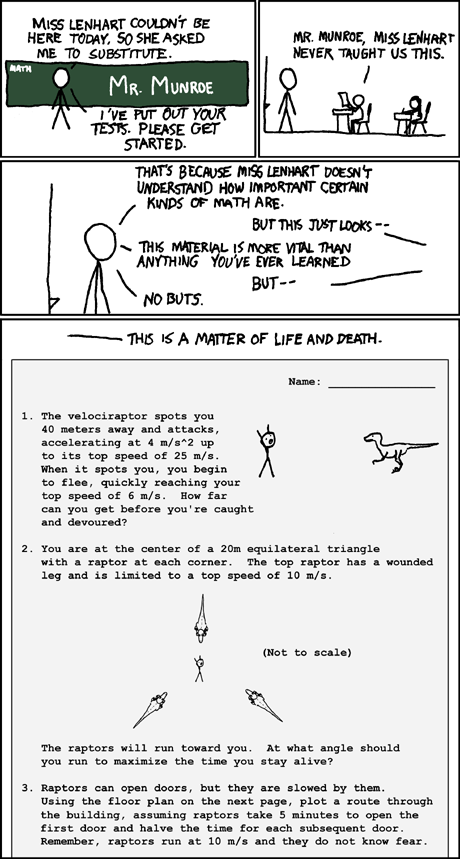
\includegraphics[scale=.57]{comics/135}
\end{center}

\end{multicols}
\subsection{Musterstudienplan für den Studiengang Lehramt Primarstufe und
Sekundarstufe I und Lehramt an der Sonderschule} 

% TODO: Anpassen
\begin{center}
\begin{tabular}{||l||l|l|l|l|l||}
\hhline{|t:=:t:=====:t|} Semester\hspace*{4mm}
    &Kürzel
    &Module\hspace*{5ex}
    &SWS\hspace*{6ex}
    &LP\hspace*{4ex}
    &Referenzsemester\hspace*{4ex} \\
\hhline{||=::=====||} 1&M1&Grundlagen der Mathematik&4+2&9&3\\
\hhline{||~||~|~|~|~|~||} &&&&&\\
\hhline{||=::=====||} 2&M2&Grundbildung Lineare Algebra und Analytische Geometrie&4+2&9&4\\
\hhline{||~||~|~|~|~|~||} &&&&&\\
\hhline{||=::=====||} 3&M3&Grundbildung Analysis&4+2&9&5\\
\hhline{||~||~|~|~|~|~||} &&&&&\\
\hhline{||=::=====||} 4&GG&Grundbildung Geometrie&2+1&5&6\\
\hhline{||~||~|~|~|~|~||} &&&&&\\
\hhline{||~||~|~|~|~|~||} &EMS&Einführung in mathematische Software&2&4&6\\
\hhline{||~||~|~|~|~|~||} &&&&&\\
\hhline{||=::=====||} 5&GS&Grundbildung Stochastik&2+1&5&6\\
\hhline{||~||~|~|~|~|~||} &&&&&\\
\hhline{||=::=====||} 6&PSEM&Proseminar&2&4&6\\
\hhline{||~||~|~|~|~|~||} &&&&&\\
\hhline{|b:=:b:=====:b|}
\end{tabular}
\end{center}
\clearpage

\begin{multicols}{2}[\section{Lehramt an Gymnasien}]

Am Fachbereich Mathematik solltest du -- zusammen mit den anderen
Mathematik-StuStudenten -- dein Studium mit Modulen aus dem
veranstaltungsgebundenen Pflichtbereich beginnen. Die Module \emphm{Analysis}
und \emphm{Lineare Algebra \& Analytische Geometrie}, welche aus den
Veranstaltungen \emphm{Analysis I} und \emphm{II} bzw. \emphm{Lineare Algebra
\& Analytische Geometrie I} und \emphm{II} bestehen, müssen im Pflichtbereich
absolviert werden. Ebenso ein \emphm{Softwarepraktikum} (SW).

Mit \emphm{Lineare Algebra \& Analytische Geometrie I} (LAAG-I) fängst du
dieses Semester schon an. Im zweiten Semester belegst du dann \emphm{Lineare
Algebra \& Analytische Geometrie II} (LAAG-II). Im dritten und vierten Semester
folgen \emphm{Analysis I} (ANA-I) und \emphm{Analysis II} (ANA-II). Die
Veranstaltungen bestehen jeweils aus 4 SWS Vorlesung, 2 SWS Übung und
freiwilligen Tutorien. Zum Ende des (zweiten bzw. vierten) Semesters schließt
du das jeweilige Modul mit einer benoteten Modulprüfung (das kann eine Klausur
oder mündliche Prüfung sein) ab.

Das unbenotete Softwarepraktikum, das 2 SWS einschließt, musst du erst während
des Masterstudiums belegen. 

Aus dem Gebiet des \emph{veranstaltungsgebundenen Pflichtbereichs} musst du
drei \emph{lehramtsspezifische Veranstaltungen} belegen, sowie ein
\emphm{Seminar} (2 SWS).  Du belegst im zweiten Semester die erste
Lehramtsspezifische Veranstaltung (LSV, Typ I) und im dritten die zweite (LSV,
Typ II).  Das Seminar (SEM) ist für das vierte Semester vorgesehen.

Je nachdem, ob Mathematik dein erstes oder dein zweites Unterrichtsfach ist,
wirst du während deines Bachelor- (wenn erstes Fach) oder während deines
Masterstudiums (wenn zweites Fach) ein \emph{Lehramtsspezifisches Projekt}
(PROJ) über 1 LP modulbegleitend absolvieren.

Im Wahlpflichtbereich wirst du vier Module (A, B, C, D) absolvieren müssen.
Davon sollten eines eine 6 LP Veranstaltung und drei 9 LP Veranstaltungen sein.
Die vier Module müssen aus dem Wahlpflichtangebot des Bachelor
Mathematik-Studienganges sein, zuzüglich der Module \emphm{Höhere Analysis},
\emphm{Numerische Mathematik} und \emphm{Mathematische Stochastik}. Wenn
Mathematik dein erstes Unterrichtsfach ist, wirst du drei dieser vier Module in
den letzten Semestern deines Bachelorstudienganges absolvieren müssen, und nur
noch eines im Masterstudium.  Ist hingegen Mathematik dein zweites
Unterrichtsfach, dann belegst du zwei der vier Module während des Bachelor- und
zwei während des Masterstudiums. Um diese Module wählen zu können, musst du in
STiNE unter Fächer/Bereichswahl die jeweiligen Gebiete auswählen. Sonst bietet
STiNE sie dir nicht zur Wahl an. Dasselbe gilt für die lehramtsspezifischen
Veranstaltungen: Die Auswahl wird sehr viel größer.

Außerdem musst du mit den Modulen A,B,C und D, den lehramtsspezifischen
Veranstaltungen und dem Seminar insgesamt 2 der Bereiche \emph{Reine
Mathematik}, \emph{Angewandte Mathematik} und \emph{Stochastik} abdecken, wenn
Mathematik dein erstes Unterrichtsfach ist. Ist Mathematik dein zweites Fach,
musst du nur einen Bereich abdecken. Im Bachelor und Master müssen alle drei
Bereiche abgedeckt werden. Im Master musst du außerdem begleitend zu einem der
Module (B,C,D) ein \emph{Lehramtsspezifisches Referat} (REF) über 2 LP halten.

\begin{center}
\vfill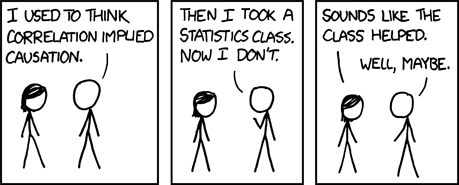
\includegraphics[scale=.9]{comics/552}
\end{center}

\clearpage
\end{multicols}
\subsection{Musterstudienplan für Lehramt Gymnasium (Bachelor und Master)}

\begin{center}
\begin{tabular}{|p{13mm}|p{40mm}||p{40mm}|p{40mm}|p{40mm}|}
\hline 				Sem. & 1.Fach Mathe & 2.Fach Mathe & SWS & LP \\
\hhline{|=|=|=|=|=|} 1.  & LAAG-I 	  & LAAG-I  	  & 6   & 9  \\
                         &            &              &     &    \\
\hline				 2.	 & LAAG-II	  & LAAG-II	 	  & 6	  & 9  \\
						       & LSV-I		  & LSV-I	     & 2	  & 3  \\
\hline				 3.	 & ANA-I		  & ANA-I	 	  & 6	  & 9  \\
						       & LSV-II     & LSV-II	     & 2   & 3  \\
\hline				 4.	 & ANA-II	  & ANA-II 	     & 6	  & 9  \\
						       & SEM  		  & SEM			  & 2	  & 3  \\
\hline				 5.	 & A		     & A	           & 6	  & 9  \\
						       & B oder D	  & B oder D	  & 4	  & 6  \\
\hline				 6.	 & D oder B	  & 	           & 6	  & 9  \\
						       & + PROJ	  & 	 	        & 	  & +1 \\
\hhline{|=|=|=|=|=|} 7.  & SW			  & SW 			  & 2	  & 4  \\
						       & 			  & 			     & 	  &    \\
\hline 				 8.    & 			  & D oder B 	  & 6	  & 9  \\
						       & 			  & + PROJ 		  & 	  & +1 \\
\hline				 9.    & C			  &              & 6	  & 9  \\
						       & + REF		  &    	        & 	  & +2 \\
\hline				 10.   & 			  & C 		     & 6   & 9  \\
                         &            & + REF        &     & +2 \\
\hline
\end{tabular}

\end{center}
\clearpage

\begin{multicols}{2}[\section{Lehramt Berufsschule}]

Da sich die einzelnen Module deines Studiengangs nicht von denen des
Studiengangs Lehramt am Gymnasium unterscheiden, können die Modulbeschreibungen
aus dem entsprechenden Artikel übernommen werden.

Auch der \emph{veranstaltungsungebundene Pflichtbereich} ist identisch zum
Lehramt Gymnasium (LAG) und besteht somit aus den Modulen \emphm{Analysis},
\emphm{Lineare Algebra und analytische Geometrie} und einem
\emphm{Softwarepraktikum}. Da ihr allerdings im Laufe eures Studiums weniger
Veranstaltungen abdecken müsst als die Studierenden des LAG, empfehlen wir euch
in den ersten beiden Semestern \emphm{Lineare Algebra und analytische Geometrie
I+II} (LA 1+2) zu hören und erst im dritten und vierten Semester
\emphm{Analysis I+II} (Ana 1+2) zu belegen. Wie die LAG-Studenten auch musst du
das \emphm{Softwarepraktikum} (SW) erst während des Masterstudiums belegen. Wir
empfehlen dir, dieses im siebten Semester zu tun.

Auch du musst zwei \emph{lehramtsspezifische Veranstaltungen} (LSV-I,II)
belegen, beide davon während deines Bachelorstudiums und empfohlen wird das
fünfte Semester. Das letzte veranstaltungsgebundene Pflichtmodul besteht auch
bei euch aus einem \emphm{Seminar} (SEM).

Im \emph{Wahlpflichtbereich} musst du nur ein Modul belegen, welches aus dem
Wahlpflichtangebot des Bachelor Mathematik-Studienganges oder aus den Modulen
\emphm{Höhere Analysis}, \emphm{Numerische Mathematik} und \emphm{Mathematische
Stochastik} stammen sollte. Du musst allerdings beachten, dass du mit diesem
Modul und dem veranstaltungsgebundenen Pflichtbereich insgesamt zwei der drei
Bereiche \emph{Stochastik}, \emph{Angewandte Mathematik} und \emph{Reine
Mathematik} abdeckst. Das Modul mit dem Wahlpflichtbereich musst du erst
während des Masterstudiums belegen, empfohlen wird hierfür das achte Semester.
Begleitend zu diesem Modul musst du wie die LAG-Studenten noch ein
lehramtsspezifisches Referat (REF) über zwei Leistungspunkte halten.

\end{multicols}
\begin{center}
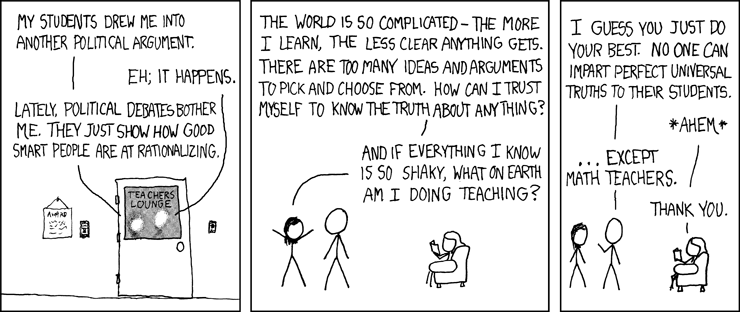
\includegraphics[scale=7]{comics/263}
\end{center}
\begin{multicols}{2}

\end{multicols}
\clearpage
\subsection{Musterstudienplan für den Studiengang Lehramt Berufliche Schulen}

\begin{center}
\begin{tabular}{||p{21mm}||p{20mm}|p{20mm}|p{20mm}|p{20mm}|p{20mm}|p{20mm}||p{20mm}|p{20mm}|p{20mm}||}

\hhline{||=||=|=|=|=|=|=||=|=|=||}& 1.Sem & 2. Sem & 3. Sem & 4. Sem & 5. Sem & 6 Sem. & 7. Sem & 8. Sem & 9./10. Sem \\ 
\hline							 gebundene& Lineare & Lineare & Analysis I & Analysis II &  &&Software-&&\\
								 Pflicht-& Algebra I & Algebra II &  & &  &&Praktikum&&\\
								 module& (9LP) & (9LP) & (9LP)& (9LP) &  &&(4LP)&&\\
\hhline{||=||=|=|=|=|=|=||=|=|=||} ungebundene& & &&& LSV, & Seminar &  &&\\
								   Pflicht-	  & & &&& Typ I& & &&\\
								   module     & & &&& (3LP)   & (3LP)   & &&\\
							   &&&&&&&&&\\
							   &&&&& LSV,&&&&\\
							   &&&&& Typ II&&&&\\
							   &&&&& (3LP) &&&&\\
\hhline{||=||=|=|=|=|=|=||=|=|=||} Wahlpflicht-&&&&&&&&Modul&\\
							   module&&&&&&&&+ Referat&\\
							   &&&&&&&& (9+2 LP)&\\
\hline						
\end{tabular}
\end{center}

\begin{multicols}{2}
